\documentclass[conference]{IEEEtran}

\usepackage[T1]{fontenc}
\usepackage[utf8]{inputenc}
\usepackage{amsmath}
\usepackage{amssymb}
\usepackage{booktabs}
\usepackage{array}
\usepackage{graphicx}
\usepackage{multirow}
\usepackage{xcolor}
\usepackage{url}
\usepackage[hidelinks]{hyperref}
\usepackage{tikz}
\usetikzlibrary{arrows.meta,positioning,shapes.geometric,fit}

\definecolor{sihatblue}{HTML}{176CA5}
\definecolor{sihatteal}{HTML}{0B8994}
\definecolor{sihatcoral}{HTML}{F26B5E}
\definecolor{sihatline}{HTML}{83BDCF}
\definecolor{sihatpaper}{HTML}{F3FBFD}

\title{SihatAI: An Inspectable Multimodal Clinical Decision-Support Workflow for Grounded, Dual-Audience Reporting in Malaysia}

\author{
\IEEEauthorblockN{S. H. Liem\textsuperscript{*} and W. L. Kher}
\IEEEauthorblockA{\textit{Veximus Technologies}\\
Selangor, Malaysia\\
\textsuperscript{*}Corresponding author: thomasliem@veximus.com.my}
}

\begin{document}
\maketitle

\begin{abstract}
Clinical information arrives as heterogeneous artifacts, including radiographs, volumetric studies, laboratory reports, longitudinal records, and spoken symptom descriptions. Converting these artifacts into usable decision support requires more than a single generative model: the surrounding system must validate inputs, protect identity, route modalities, structure outputs, ground claims, expose uncertainty, preserve human oversight, and communicate differently to clinicians and patients. This paper presents SihatAI, an inspectable multimodal clinical decision-support system designed for the Malaysian healthcare context. The production path combines a Laravel and Vue clinical application with a FastAPI inference service and Modal-hosted MedGemma 1.5 4B inference with Malaysia-oriented MY-LoRA adaptation loaded at serve time through PEFT. A canonical findings object separates evidence extraction from audience-specific communication. The implemented workflow includes heuristic and vision-model-assisted routing, imaging and document specialist hops with partial-findings merge, DICOM and PDF preprocessing, optical character recognition, prompted structured generation, hybrid BM25 and dense retrieval with maximal marginal relevance, sibling safe-URI de-identification, ALLOW/WARN safety policies with audit events and clinician notification, physician sign-gated patient release, longitudinal comparison, similar-case retrieval, MedASR with Whisper fallback, multilingual templates, and an evaluation regression gate. We describe the algorithms and software contracts of the live system. We also distinguish model-reported confidence from calibrated probability, prompted boxes from validated detection, slice montages from volumetric reasoning, and software verification from clinical validation. Current evidence establishes production workflow completeness, not diagnostic efficacy. The paper contributes a reproducible architecture, an explicit claim boundary, and an evaluation roadmap for clinical, multilingual, calibration, privacy, and human-factors studies.
\end{abstract}

\begin{IEEEkeywords}
clinical decision support, multimodal artificial intelligence, vision-language model, MedGemma, retrieval-augmented generation, medical imaging, DICOM, optical character recognition, human oversight, Malaysia
\end{IEEEkeywords}

\section{Introduction}

Healthcare data are intrinsically multimodal. A clinical episode may include a chest radiograph, a computed tomography (CT) series, a laboratory panel, a prior report, medication and symptom history, and a spoken account from the patient. These artifacts are generated by different devices and workflows, stored in different representations, and interpreted by people with different information needs. A radiologist needs technical detail and uncertainty; a patient needs a clear explanation and an actionable next step. A system that only produces fluent prose does not resolve this fragmentation. It must preserve the relationship between an output and the evidence that produced it.

The Malaysian setting makes this problem particularly relevant. The Ministry of Health Malaysia has identified staged electronic medical record and electronic lifetime health record deployment as part of national health-system reform \cite{moh2023whitepaper}. The Malaysia Health Reference Data Model similarly emphasizes interoperable, consistent data across the continuum of care \cite{mohmyhrdm}. At the same time, Malaysia has reported a low radiologist-to-population ratio relative to several higher-income systems, with uneven geographic distribution \cite{ramli2023radiologist}. Communication is also a systems problem. Malaysia is multilingual, and national health-literacy research identifies meaningful variation associated with age, education, and income \cite{jaafar2021literacy}; qualitative work further shows that language and distributed support affect how multi-ethnic patients manage health information \cite{rajan2021multilingual}.

Large multimodal models can accept images and text and produce flexible textual outputs. MedGemma 1.5 is a medically adapted 4-billion-parameter multimodal model based on Gemma 3 \cite{sellergren2026medgemma,gemmateam2025gemma3}. Its supported capabilities create a useful foundation for prototyping medical image understanding, document extraction, localization, and longitudinal reasoning. However, a foundation model is not a complete clinical product. Model outputs may be unsupported, incorrectly localized, overconfident, or difficult to audit. World Health Organization guidance therefore places autonomy, safety, transparency, accountability, inclusiveness, and sustainability at the center of health AI governance \cite{who2021ethics}; its guidance for large multimodal models adds specific concern about inaccurate content, automation bias, cybersecurity, and post-release auditing \cite{who2024lmm}.

SihatAI was developed around the proposition that the clinical workflow surrounding the model is as important as the model itself. It is a production decision-support system, not an autonomous diagnostic device. The system accepts supported medical artifacts, converts them into a canonical findings object, applies hybrid retrieval and ALLOW/WARN policy checks, and derives two reports: a technical physician-facing draft and a patient-facing explanation released only after physician sign-off when policy allows. It retains the original and scrubbed artifacts for review and exposes pipeline stages, engine and adapter labels, citations, confidence labels, visual overlays, audit events, and sign-off state.

This paper makes four contributions:

\begin{enumerate}
    \item It specifies an end-to-end, live-first clinical workflow that separates the web application, asynchronous orchestration, Modal-hosted model inference, and post-inference safety processing through a signed contract.
    \item It introduces a canonical findings object as the shared evidence layer for physician and patient reports, preventing audience adaptation from silently changing the underlying findings.
    \item It documents an inspectable policy layer for hybrid retrieval strength, confidence bands, critical-value escalation with audit and notify, WARN veto of patient prose, longitudinal comparison, and sign-gated patient release.
    \item It provides an explicit claim boundary. Production software completeness, including hybrid RAG, specialist hops, MedASR, and implemented MY-LoRA adaptation, is separated from clinical accuracy so that engineering maturity is not presented as diagnostic efficacy.
\end{enumerate}

The remainder of the paper reviews the technical foundations, presents the system and algorithms, describes implementation and verification, and develops a rigorous evaluation and deployment roadmap.

\section{Background and Related Work}

\subsection{Medical Multimodal Models}

Vision-language models (VLMs) combine visual encoders with language models to answer questions or generate text conditioned on images. Radiology-focused systems such as MAIRA-1 demonstrate that domain-specific visual and language adaptation can improve report generation, while also exposing errors that conventional lexical metrics may not capture \cite{bannur2024maira1}. MAIRA-2 extends the task toward grounded reporting with current and prior views, prior reports, and explicit localization \cite{bannur2024maira2}. These studies reinforce two design lessons relevant to SihatAI. First, context and prior evidence matter. Second, generated localization and narrative require task-specific evaluation against expert references. Public chest radiograph corpora such as MIMIC-CXR support standardized imaging evaluation with paired reports \cite{johnson2019mimiccxr}, but SihatAI does not yet report results on that or any external clinical benchmark.

MedGemma 1.5 provides a unified open model for medical text and image comprehension, including high-dimensional imaging, histopathology, localization, longitudinal imaging, and document understanding \cite{sellergren2026medgemma,googlemedgemmacard}. SihatAI uses the instruction-tuned 4B checkpoint through prompted structured generation. It does not train a dedicated detector, segmenter, or modality-specific classification head. Consequently, its bounding boxes are generative coordinates requested in a JSON prompt, and its CT, magnetic resonance imaging (MRI), and histopathology inputs are reduced to two-dimensional montages. These distinctions are central to the paper's claim boundary.

\subsection{Retrieval and Grounded Generation}

Retrieval-augmented generation (RAG) combines parametric generation with a non-parametric corpus, enabling outputs to be conditioned on retrieved evidence and permitting knowledge to be updated without full model retraining \cite{lewis2020rag}. Retrieval can use dense vector similarity, sparse lexical methods, or both. BM25 is a probabilistic sparse retrieval framework that performs well when query and document terms overlap \cite{robertson2009bm25}. Maximal marginal relevance (MMR) can rerank results by balancing query relevance against redundancy \cite{carbonell1998mmr}.

SihatAI implements a hybrid RAG stack over Ministry of Health guideline chunks. Dense cosine retrieval over external embeddings or a deterministic 64-dimensional hashed bag-of-tokens representation is fused with an in-process BM25 candidate set, then reranked with maximal marginal relevance (MMR; \(\lambda=0.7\)) to return the top three citations. When the corpus is empty or the top fused score is weak, the live path returns empty citations and records weak grounding rather than inserting static stubs. Source-version governance and claim-to-citation entailment remain future work; unsupported recommendations must still abstain rather than invent support.

\subsection{Parameter-Efficient Adaptation}

Low-Rank Adaptation (LoRA) freezes the base model and introduces trainable low-rank matrices, reducing trainable parameter count and deployment storage \cite{hu2022lora}. QLoRA extends this approach by back-propagating through a frozen 4-bit quantized model into LoRA adapters \cite{dettmers2023qlora}. SihatAI implements MY-LoRA end to end: curated JSONL splits (approximately 4842 train and 538 validation chat examples from Malaysian guideline and communication material), Modal QLoRA training, shipped adapter weights, and inference-time PEFT load via \texttt{SIHAT\_AI\_LORA\_PATH}. Served responses label the loaded adapter. The adaptation targets Malaysian clinical guideline language and dual-audience reporting style on MedGemma, while live multimodal inference remains image-to-text with the adapted model. This paper reports the implemented adaptation path as part of the production system; separate clinical outcome trials are outside the present software contribution.

\subsection{Uncertainty, Abstention, and Oversight}

Modern neural networks may be poorly calibrated, meaning a reported confidence does not correspond to empirical correctness probability \cite{guo2017calibration}. A selective prediction system can reject or defer uncertain cases, but effective rejection requires uncertainty estimates that are valid for the target population and task \cite{geifman2019selectivenet}. SihatAI currently applies fixed policy thresholds to model-reported values. It has not fitted temperature scaling, evaluated expected calibration error (ECE), computed Brier scores, or estimated risk-coverage curves. Its mechanism should therefore be described as \emph{heuristic confidence gating}, not calibrated uncertainty.

Human review is similarly more than a disclaimer. Automation bias can lead users to overvalue polished machine outputs \cite{cabitza2017unintended}. SihatAI keeps the original artifact visible, labels the output as decision support, allows physicians to amend a draft, and records a signed snapshot. These are workflow controls; they do not prove that users will detect errors. Future evaluation should follow early-stage clinical reporting guidance such as DECIDE-AI \cite{vasey2022decideai} and imaging-specific reporting guidance such as CLAIM \cite{mongan2020claim}.

\section{System Scope and Design Principles}

\subsection{Intended Use}

SihatAI is intended for clinician-supervised decision support in production-configured deployments. Supported tasks include artifact ingestion, preliminary structured findings, biomarker extraction, guideline-oriented hybrid retrieval, longitudinal summaries, patient-friendly communication, and workflow review. Prohibited reliance includes autonomous diagnosis, autonomous treatment or prescribing, emergency dispatch, final clinical reporting without authorized review, and processing identifiable health information outside an approved environment.

The system has two authenticated roles. Physicians can review records, upload on behalf of a patient, edit unsigned draft reports, sign a snapshot that gates patient release, inspect similar cases, and run evaluation suites. Patients can view only their own records and patient-facing reports, subject to WARN withholding and unsigned drafts. Registration is disabled in the current deployment configuration; authentication, password reset, email verification, role middleware, policies, and rate limiting are provided by Laravel Fortify.

\subsection{Design Principles}

Five principles shape the implementation:

\begin{enumerate}
    \item \textbf{Evidence before prose.} Structured findings are created before physician and patient reports.
    \item \textbf{One findings object, multiple presentations.} Audience and language adaptation operate on the same findings object.
    \item \textbf{Fail visibly.} Pipeline stages, failure state, retrieval weakness, and withholding reasons are represented in persistent state.
    \item \textbf{Human authority.} A clinician can inspect the source, edit the draft, and sign a snapshot; the AI does not issue an independent final diagnosis.
    \item \textbf{Claim proportionality.} Demonstration fallbacks and unvalidated algorithms remain explicitly labeled.
\end{enumerate}

\section{Architecture}

SihatAI uses a decoupled application and inference architecture (Fig.~\ref{fig:architecture}). The application tier is built with Laravel 13, MySQL, a database-backed queue, Inertia, and Vue. The inference tier is a FastAPI service that performs file preparation and calls a Modal GPU endpoint hosting MedGemma with MY-LoRA and MedASR with Whisper fallback. A job identifier and record identifier correlate all stages. The FastAPI service returns asynchronously through a Hypertext Transfer Protocol (HTTP) webhook protected by a Hash-based Message Authentication Code using SHA-256 (HMAC-SHA256). Live inference is the default (\texttt{SIHAT\_AI\_USE\_MOCK=false}). A deterministic offline harness remains available only when automated tests or operators explicitly enable it.

\begin{figure*}[t]
\centering
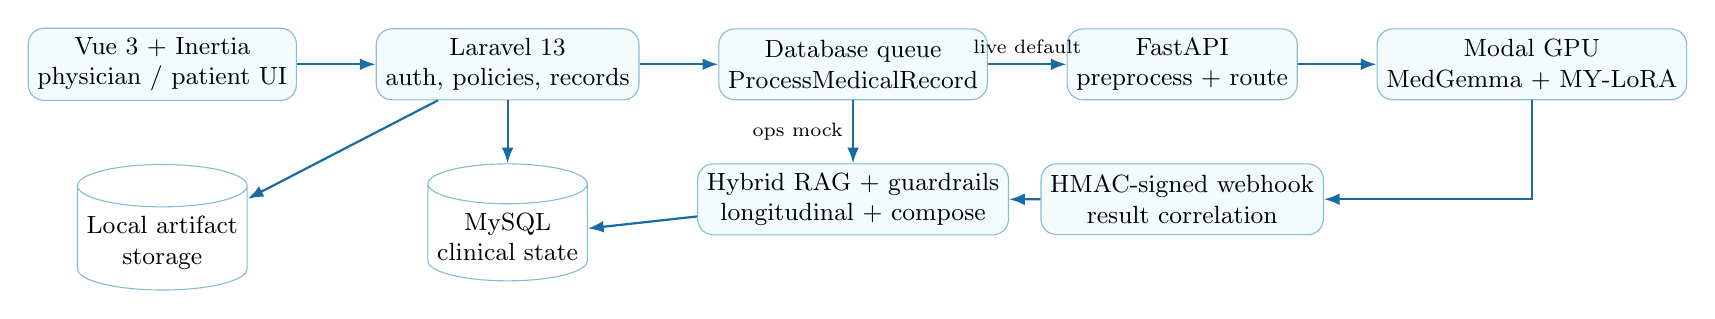
\begin{tikzpicture}[
  node distance=8mm and 10mm,
  box/.style={draw=sihatline, rounded corners=2mm, fill=sihatpaper, minimum height=9mm, align=center, font=\small},
  store/.style={draw=sihatline, cylinder, shape border rotate=90, aspect=0.25, fill=white, minimum height=11mm, align=center, font=\small},
  arrow/.style={-{Latex[length=2mm]}, thick, draw=sihatblue}
]
\node[box] (ui) {Vue 3 + Inertia\\physician / patient UI};
\node[box, right=of ui] (laravel) {Laravel 13\\auth, policies, records};
\node[box, right=of laravel] (queue) {Database queue\\ProcessMedicalRecord};
\node[box, right=of queue] (fastapi) {FastAPI\\preprocess + route};
\node[box, right=of fastapi] (modal) {Modal GPU\\MedGemma + MY-LoRA};
\node[box, below=of fastapi] (webhook) {HMAC-signed webhook\\result correlation};
\node[box, below=of queue] (finalize) {Hybrid RAG + guardrails\\longitudinal + compose};
\node[store, below=of laravel] (db) {MySQL\\clinical state};
\node[store, below=of ui] (disk) {Local artifact\\storage};

\draw[arrow] (ui) -- (laravel);
\draw[arrow] (laravel) -- (queue);
\draw[arrow] (queue) -- node[above,font=\scriptsize]{live default} (fastapi);
\draw[arrow] (fastapi) -- (modal);
\draw[arrow] (modal) |- (webhook);
\draw[arrow] (webhook) -- (finalize);
\draw[arrow] (queue) -- node[left,font=\scriptsize]{ops mock} (finalize);
\draw[arrow] (finalize) -- (db);
\draw[arrow] (laravel) -- (db);
\draw[arrow] (laravel) -- (disk);
\end{tikzpicture}
\caption{SihatAI architecture. The default path is live FastAPI and Modal inference with a signed webhook. An explicit mock flag remains for tests and controlled offline runs.}
\label{fig:architecture}
\end{figure*}

\subsection{Artifact Lifecycle}

An uploaded file is validated by extension and size, stored on a local private disk, and represented by a \texttt{medical\_records} row. Supported extensions are JPEG, PNG, PDF, DICOM, and ZIP, with a 50 MB request limit. An \texttt{analysis\_jobs} row stores execution state. The record status advances from pending to processing and then completed or failed. JSON columns preserve findings, reports, citations, boxes, guardrail flags (including ALLOW/WARN), pipeline steps, traces, partial findings, embeddings, volume metadata, patch metadata, safe-file path, and signature data. Biomarkers are normalized into a separate relational table so that values can be trended. Durable \texttt{audit\_events} capture critical escalations.

The pipeline stages are upload, de-identification to a sibling scrubbed artifact, routing, analysis with imaging and document specialist hops, hybrid retrieval, guardrail evaluation, and composition (Fig.~\ref{fig:pipeline}). The code records a hop trace with \texttt{partial\_findings} merge. The term ``agent'' in the user interface refers to these bounded, inspectable stages; specialist hops follow a parallel contract while execution remains sequential in the current service.

\begin{figure*}[t]
\centering
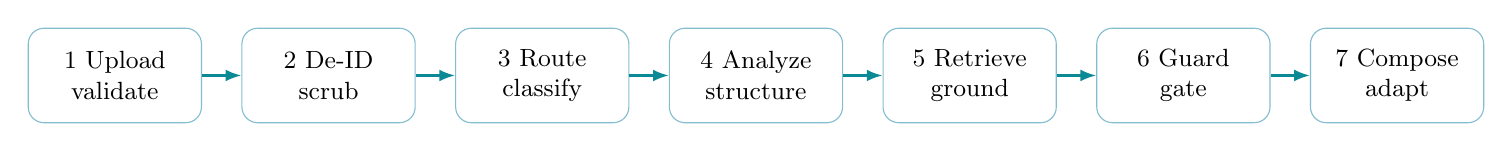
\begin{tikzpicture}[
  stage/.style={draw=sihatline, rounded corners=2mm, fill=white, minimum width=22mm, minimum height=12mm, align=center, font=\small},
  arrow/.style={-{Latex[length=2mm]}, thick, draw=sihatteal}
]
\node[stage] (s1) {1 Upload\\validate};
\node[stage, right=5mm of s1] (s2) {2 De-ID\\scrub};
\node[stage, right=5mm of s2] (s3) {3 Route\\classify};
\node[stage, right=5mm of s3] (s4) {4 Analyze\\structure};
\node[stage, right=5mm of s4] (s5) {5 Retrieve\\ground};
\node[stage, right=5mm of s5] (s6) {6 Guard\\gate};
\node[stage, right=5mm of s6] (s7) {7 Compose\\adapt};
\foreach \a/\b in {s1/s2,s2/s3,s3/s4,s4/s5,s5/s6,s6/s7}
  \draw[arrow] (\a) -- (\b);
\end{tikzpicture}
\caption{Sequential, logged pipeline stages. The implementation records hop metadata but does not run parallel specialists.}
\label{fig:pipeline}
\end{figure*}

\subsection{Remote Inference Contract}

In live mode, Laravel sends a POST request to \texttt{/api/v1/analyze}. The payload contains the job and record identifiers, initial modality, language, MIME type, original filename, route confidence, a temporary signed file URL, and a callback URL. FastAPI accepts the request and starts a background task. It downloads the file through the signed URL, performs modality-specific preparation, and calls the Modal endpoint. Completion is returned to Laravel as JSON with a signature

\begin{equation}
    \sigma = \operatorname{HMAC}_{\mathrm{SHA256}}(k, b),
\end{equation}

where \(k\) is the shared secret and \(b\) is the exact request body. Laravel computes the same value and performs a constant-time comparison before accepting the result. This protects callback authenticity. Critical outcomes additionally write durable audit events and notify the uploading physician. Production hardening should still add nonce or timestamp validation, key rotation procedures, and transport controls.

\section{Technical Methods}

\subsection{De-Identification}

The application performs a pre-inference scrub and writes a sibling artifact under \texttt{medical-records/safe/}, persisted as \texttt{safe\_file\_path}. Filename and extracted text patterns redact Malaysian identity-number-like strings, telephone numbers, email addresses, medical record numbers, and simple patient-name labels. JPEG and PNG files are decoded and re-encoded to remove metadata when the required image functions are available. DICOM files receive a binary keyword replacement pass for common attributes. The AI file route serves the scrubbed sibling to remote inference when present.

This method reduces obvious disclosure but is not a standards-conformant DICOM de-identifier. DICOM PS3.15 Annex E defines attribute confidentiality profiles, actions for nested data sets, and optional handling for pixel data, descriptors, dates, device identity, and private tags \cite{dicom2026ps315}. The standard itself notes that attribute processing alone does not guarantee de-identification of the information object. SihatAI does not yet remove burned-in annotations, evaluate re-identification risk, or assert PS3.15 conformance. For these reasons the manuscript uses the term \emph{pattern-based pre-inference scrubbing with a sibling safe URI}.

\subsection{Modality Routing}

Routing begins with MIME type, extension, and filename features. Laboratory PDFs and clinical documents (for example discharge or clinic notes) are distinguished by filename hints. Specific keywords identify ophthalmology, dermatology, histopathology, CT, MRI, or radiography. DICOM content can be recognized from the \texttt{DICM} preamble and selected metadata. The system assigns a heuristic route confidence, commonly 0.85 for a keyword match and 0.95 for PDF routing.

When an image route is absent or below 0.70 and Modal is available, the image is sent to MedGemma with a constrained zero-shot classification prompt. The returned class must be in the supported set; an unrecognized class falls back to radiography with confidence at most 0.50. This is a deterministic workflow heuristic augmented by VLM classification. It is not a trained routing model, and no confusion matrix is currently reported.

\subsection{DICOM and Volume Preparation}

DICOM processing uses pydicom and NumPy. A data set is decoded with transfer-syntax support supplied by pylibjpeg plugins where available. Single-frame arrays and multi-frame arrays are normalized into a sequence. For grayscale frames, the implementation first applies window center \(c\) and width \(w\), when present:

\begin{equation}
  I_c = \operatorname{clip}\left(I, c-\frac{w}{2}, c+\frac{w}{2}\right).
\end{equation}

The resulting values are linearly scaled to 8-bit intensity:

\begin{equation}
  I_8 = 255\frac{I_c-\min(I_c)}{\max(I_c)-\min(I_c)}.
\end{equation}

\texttt{MONOCHROME1} images are inverted, and grayscale values are replicated into three RGB channels. If a study contains multiple frames, the implementation chooses at most eight consecutive indices centered approximately on the midpoint. ZIP archives are sorted by name and sampled using the same midpoint strategy. Selected images are resized to the smallest tile dimensions and placed in a grid. The montage is encoded as JPEG and supplied to the VLM.

This process is computationally simple and enables multi-slice input summarization. It discards full spatial geometry, slice spacing, orientation, acquisition phase, and potentially informative peripheral slices. It is therefore described as \emph{mid-slice montage summarization}, not three-dimensional analysis or reconstruction.

\subsection{Histopathology Preparation}

For a conventional image representing a histopathology specimen, the system crops the central 60\% of width and height, divides the crop into a \(3\times3\) grid, and composes the nine patches into a montage. Each patch receives a row-column identifier. The same MedGemma image method processes this montage.

The method does not use OpenSlide, magnification-aware sampling, tissue masking, stain normalization, a whole-slide pyramid, multiple-instance learning, or slide-level aggregation. It supports patch-referenced output but cannot support a whole-slide diagnostic claim.

\begin{figure*}[t]
\centering
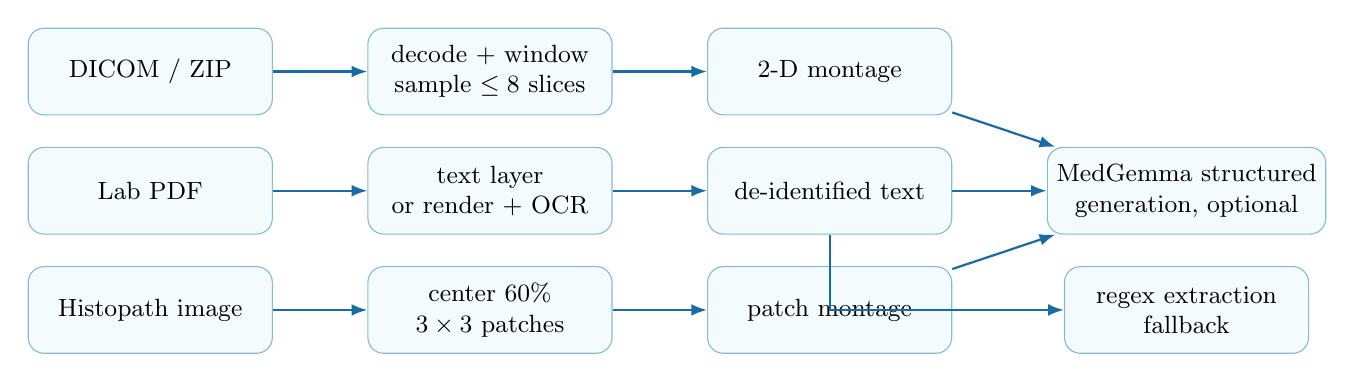
\begin{tikzpicture}[
  box/.style={draw=sihatline, rounded corners=2mm, fill=sihatpaper, minimum width=31mm, minimum height=11mm, align=center, font=\small},
  arrow/.style={-{Latex[length=2mm]}, thick, draw=sihatblue}
]
\node[box] (dicom) {DICOM / ZIP};
\node[box, below=4mm of dicom] (pdf) {Lab PDF};
\node[box, below=4mm of pdf] (histo) {Histopath image};

\node[box, right=12mm of dicom] (dprep) {decode + window\\sample $\leq8$ slices};
\node[box, right=12mm of pdf] (pprep) {text layer\\or render + OCR};
\node[box, right=12mm of histo] (hprep) {center 60\%\\$3\times3$ patches};

\node[box, right=12mm of dprep] (dm) {2-D montage};
\node[box, right=12mm of pprep] (pt) {de-identified text};
\node[box, right=12mm of hprep] (hm) {patch montage};

\node[box, right=12mm of pt] (model) {MedGemma structured\\generation, optional};
\node[box, below=4mm of model] (rules) {regex extraction\\fallback};

\draw[arrow] (dicom) -- (dprep);
\draw[arrow] (pdf) -- (pprep);
\draw[arrow] (histo) -- (hprep);
\draw[arrow] (dprep) -- (dm);
\draw[arrow] (pprep) -- (pt);
\draw[arrow] (hprep) -- (hm);
\draw[arrow] (dm) -- (model);
\draw[arrow] (pt) -- (model);
\draw[arrow] (hm) -- (model);
\draw[arrow] (pt) |- (rules);
\end{tikzpicture}
\caption{Modality-specific preprocessing. Volume and pathology branches produce two-dimensional montages; document processing prefers a native text layer before OCR.}
\label{fig:preprocessing}
\end{figure*}

\subsection{Laboratory PDF Extraction}

The laboratory path first attempts embedded text extraction using pypdf and PyMuPDF. If the resulting layer contains fewer than 40 non-whitespace characters, each of at most four pages is rendered at scale 2.0 and passed to RapidOCR, an ONNX Runtime-based OCR library \cite{rapidocr}. Tesseract can act as an optional fallback when installed. Extracted text is scrubbed for common identity patterns before analysis.

When live MedGemma is available, a constrained text prompt requests arrays of findings and biomarkers. Otherwise, a rule-based parser searches for 13 configured analytes, including hemoglobin, platelets, white and red blood cells, creatinine, glucose, glycated hemoglobin, liver enzymes, sodium, and potassium. For analyte \(a\) with extracted value \(v_a\) and configured interval \([l_a,h_a]\), the fallback assigns

\begin{equation}
s_a=
\begin{cases}
\mathrm{normal}, & l_a\le v_a\le h_a,\\
\mathrm{critical}, & v_a<0.7l_a\ \mathrm{or}\ v_a>1.4h_a,\\
\mathrm{abnormal}, & \mathrm{otherwise}.
\end{cases}
\end{equation}

These reference intervals are fixed constants, not laboratory-specific clinical ranges. Real deployment must preserve the source report's ranges, units, specimen context, patient characteristics, and laboratory methodology. The regex also allows a broad non-digit gap between label and value, which helps with OCR line breaks but can associate the wrong value in complex tables.

\subsection{MedGemma Structured Generation}

The Modal image loads \texttt{google/medgemma-1.5-4b-it} using the Hugging Face processor and image-to-text model class. Weights use bfloat16 with automatic device placement on an L4 GPU. MY-LoRA is loaded over the base model through PEFT using the configured adapter path. Inference uses a chat template and greedy decoding:

\begin{equation}
 y_t = \arg\max_{v \in V} p(v \mid x_\mathrm{image},x_\mathrm{text},y_{<t}),
\end{equation}

with sampling disabled and a maximum of 1200 new tokens for image analysis. The prompt requests JSON containing findings, differential diagnoses, overall confidence, and normalized boxes. Laboratory text uses a related schema that also requests structured biomarkers.

The service attempts strict JSON parsing, then extracts the first brace-delimited object if needed. If parsing still fails, the raw narrative is wrapped as one borderline finding with a score of 0.60. Coordinates are clamped to \([0,1]\), width and height are constrained to remain inside the image, boxes smaller than 0.01 in either dimension are discarded, and at most eight boxes are retained.

This approach is \emph{prompted structured generation}. It does not guarantee schema validity, factuality, or localization quality. The confidence fields are generated tokens. The postprocessor enforces numerical bounds but cannot determine whether the region corresponds to the finding.

\subsection{Retrieval over Guideline Chunks}

The query concatenates current finding labels, up to three prior-record labels for the same patient, and the modality label. Guideline chunks are stored in MySQL with source, section, content, and an optional embedding. With an external embedding service configured, SihatAI requests \texttt{text-embedding-3-small}. Otherwise it uses a deterministic local hash representation. For lowercase tokens \(t\), a 64-dimensional vector is formed as

\begin{equation}
  z_j = \sum_{t:\,\mathrm{crc32}(t)\bmod64=j} 1,\qquad
  \hat{\mathbf z} = \frac{\mathbf z}{\|\mathbf z\|_2}.
\end{equation}

Dense candidates use cosine similarity:

\begin{equation}
 \operatorname{sim}(\mathbf q,\mathbf d)=
 \frac{\mathbf q^\top\mathbf d}{\|\mathbf q\|_2\|\mathbf d\|_2}.
\end{equation}

In parallel, an in-process BM25 scorer ranks the same corpus with \(k_1=1.2\) and \(b=0.75\), and scores are normalized into approximately \([0,1]\). Dense and BM25 candidate lists (top eight each) are fused by source-section key, with a small boost when both retrievers select the same chunk. Maximal marginal relevance then selects the final top \(k=3\) citations:

\begin{equation}
\operatorname{MMR}(d)=
\lambda\,\mathrm{rel}(d)-(1-\lambda)\max_{d'\in S}\mathrm{sim}(d,d'),
\end{equation}

with \(\lambda=0.7\). Retrieval is flagged weak when the top fused score is below 0.20 or no candidates remain. In that case the live path returns empty citations and records weak grounding; static stubs are not injected into production reports. The offline hash embedding is inexpensive and reproducible but has collisions and limited semantics; BM25 therefore carries much of the offline signal. Source-version governance and claim-to-citation entailment remain future work.

\subsection{Similar Cases and Longitudinal Comparison}

Similar-case retrieval embeds the modality and finding labels of a completed record and compares them with at most 50 recent completed records. Cosine similarity is used when embeddings are available; lexical term overlap is the fallback. A same-modality candidate receives a 0.05 score bonus, capped at 1.0. This is text-label similarity over the deployed record bank, not image similarity and not an epidemiological estimate.

Longitudinal comparison selects a prior record from the same patient and modality. Imaging findings are compared by normalized label sets to classify labels as new, stable, or resolved. Laboratory values are compared by analyte name and numeric difference. These are deterministic summaries. They do not model uncertainty, measurement error, clinical directionality, or treatment context.

\subsection{Safety Policy}

The post-inference policy reads overall model-reported confidence \(c\), critical biomarker flags, and retrieval weakness. The confidence decision is

\begin{equation}
g(c)=
\begin{cases}
\mathrm{publish}, & c\ge0.80,\\
\mathrm{hedge}, & 0.50\le c<0.80,\\
\mathrm{abstain}, & c<0.50.
\end{cases}
\end{equation}

Policy state is summarized as \texttt{ALLOW} or \texttt{WARN}. A critical value adds an escalation flag, writes an \texttt{audit\_events} row, and notifies the uploading physician by mail. Abstention, critical values, or \texttt{WARN} prevent composition of patient-facing model prose. Patient release additionally requires physician \texttt{signed\_at}. The physician view retains findings, warnings, and source artifacts for review. Figure~\ref{fig:guardrail} summarizes the state logic.

\begin{figure}[t]
\centering
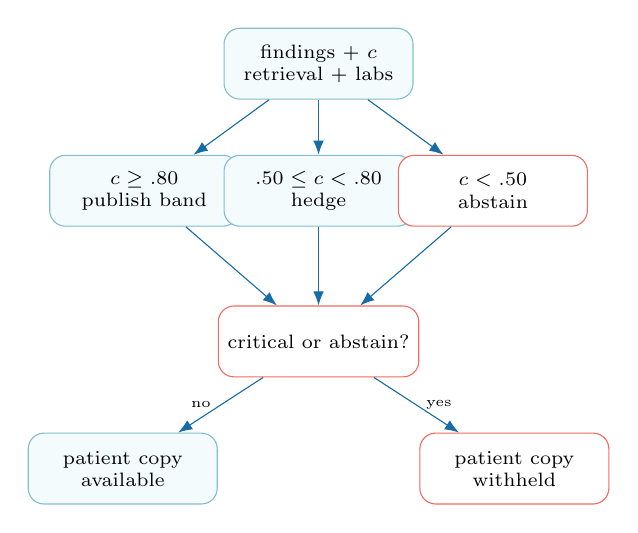
\begin{tikzpicture}[
  state/.style={draw=sihatline, rounded corners=2mm, fill=sihatpaper, minimum width=24mm, minimum height=9mm, align=center, font=\scriptsize},
  alert/.style={draw=sihatcoral, rounded corners=2mm, fill=white, minimum width=24mm, minimum height=9mm, align=center, font=\scriptsize},
  arrow/.style={-{Latex[length=1.8mm]}, draw=sihatblue}
]
\node[state] (input) {findings + \(c\)\\retrieval + labs};
\node[state, below left=7mm and -2mm of input] (pub) {\(c\geq.80\)\\publish band};
\node[state, below=7mm of input] (hedge) {\(.50\leq c<.80\)\\hedge};
\node[alert, below right=7mm and -2mm of input] (abstain) {\(c<.50\)\\abstain};
\node[alert, below=10mm of hedge] (critical) {critical or abstain?};
\node[state, below left=7mm and 0mm of critical] (patient) {patient copy\\available};
\node[alert, below right=7mm and 0mm of critical] (withhold) {patient copy\\withheld};
\draw[arrow] (input) -- (pub);
\draw[arrow] (input) -- (hedge);
\draw[arrow] (input) -- (abstain);
\draw[arrow] (pub) -- (critical);
\draw[arrow] (hedge) -- (critical);
\draw[arrow] (abstain) -- (critical);
\draw[arrow] (critical) -- node[left,font=\tiny]{no} (patient);
\draw[arrow] (critical) -- node[right,font=\tiny]{yes} (withhold);
\end{tikzpicture}
\caption{Policy gating. Thresholds operate on model-reported scores and must not be interpreted as calibrated empirical probabilities. WARN and unsigned drafts block patient release.}
\label{fig:guardrail}
\end{figure}

\subsection{One Findings Object, Two Reports}

The canonical object contains finding label, description, severity, confidence, optional box, biomarkers and reference intervals, differential suggestions, longitudinal changes, citations, engine and adapter labels, and policy state. The system then uses PHP templates to compose physician and patient reports in English, Bahasa Melayu, Mandarin, or Tamil (Fig.~\ref{fig:dualreport}). The physician version preserves technical findings, differential suggestions, confidence, citations, and review notes. The patient version uses simpler phrasing and an action-oriented next step. If policy requires withholding or the draft is unsigned, the patient receives a controlled message rather than the full generated report.

\begin{figure}[t]
\centering
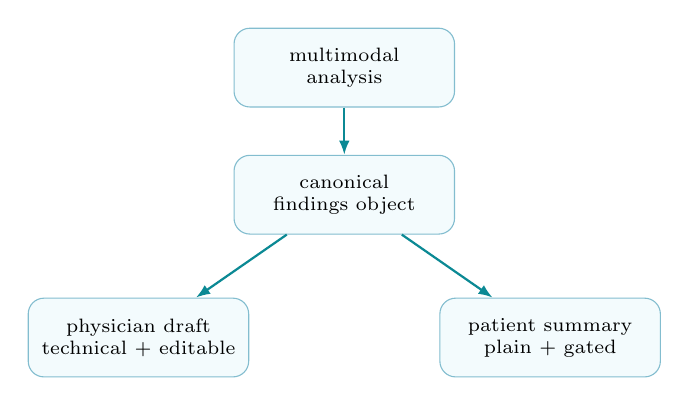
\begin{tikzpicture}[
  box/.style={draw=sihatline, rounded corners=2mm, fill=sihatpaper, minimum width=28mm, minimum height=10mm, align=center, font=\scriptsize},
  arrow/.style={-{Latex[length=1.8mm]}, thick, draw=sihatteal}
]
\node[box] (source) {multimodal\\analysis};
\node[box, below=6mm of source] (object) {canonical\\findings object};
\node[box, below left=8mm and -2mm of object] (phys) {physician draft\\technical + editable};
\node[box, below right=8mm and -2mm of object] (pat) {patient summary\\plain + gated};
\draw[arrow] (source) -- (object);
\draw[arrow] (object) -- (phys);
\draw[arrow] (object) -- (pat);
\end{tikzpicture}
\caption{Audience adaptation changes presentation, not the evidence object. Current reports are template-based rather than separately generated by MedGemma.}
\label{fig:dualreport}
\end{figure}

This separation limits one class of inconsistency because the two outputs do not invoke independent image inference. It does not prove semantic equivalence across languages. Clinical translation and simplification must be evaluated by qualified multilingual reviewers.

\subsection{Voice Triage}

The voice path sends base64-encoded audio to FastAPI, which prefers Google MedASR on a Modal T4 GPU and falls back to Whisper base when MedASR cannot be loaded \cite{radford2023whisper}. The response labels the active \texttt{engine}. If speech recognition is unavailable, the service returns an empty fallback and asks for text. Browser \texttt{speechSynthesis} provides minimal text-to-speech interview prompts. The Laravel controller structures urgency using keyword rules and can optionally ask a general language model for JSON. The result is routine, urgent, or emergency guidance with follow-up prompts.

This path is an accessibility-oriented intake aid. It is not a clinically validated triage model and not emergency dispatch. Word error rate, language-specific performance, code-switching, accent robustness, urgency sensitivity, and false-reassurance risk remain unevaluated.

\section{Implementation}

\subsection{Application Tier}

The application uses PHP 8.4 and Laravel 13 \cite{laravel13}. Laravel manages sessions, Fortify authentication, email verification, authorization policies, validation, storage, relational state, jobs, signed URLs, and webhook handling. MySQL stores users, medical records, analysis jobs, biomarkers, guideline chunks, and evaluation runs. The development queue uses the database driver, and artifacts use private local storage.

The interface uses Vue 3, TypeScript, Inertia 3, Laravel Wayfinder, Tailwind CSS 4, shadcn-vue primitives, Reka UI, and Vite. Physician screens prioritize scan overlays, compact findings, citations, traces, and report controls. Patient screens emphasize plain-language summaries, trends, and large action targets. Normalized box coordinates are rendered over the displayed image; they remain visual aids and do not alter source pixels.

\subsection{Inference Tier}

The local inference service uses Python, FastAPI, Pydantic, Uvicorn, and HTTPX \cite{fastapi}. Pydantic validates request fields and response shape at the service boundary. PyMuPDF and pypdf extract or render PDF content; RapidOCR and ONNX Runtime handle OCR; pydicom, pylibjpeg, NumPy, and Pillow decode and prepare images.

The Modal image adds PyTorch, Transformers, Accelerate, PEFT, MedASR, and OpenAI Whisper. MedGemma with MY-LoRA uses an L4 GPU and speech recognition uses a T4 GPU. Cloud serving is the production inference path; local requirements omit large model weights. Training used TRL, bitsandbytes, Datasets, and related tooling for the MY-LoRA QLoRA run on Modal.

\subsection{Operational Modes}

Table~\ref{tab:modes} distinguishes the operational modes. The default application configuration is live: FastAPI, Modal MedGemma with MY-LoRA, a queue worker, Hugging Face credentials, and matching webhook secrets. A deterministic offline harness exists only when \texttt{SIHAT\_AI\_USE\_MOCK=true} for automated tests or controlled offline operation. Responses persist honest \texttt{engine} and \texttt{adapter} labels so offline or base-model runs are not branded as adapted MedGemma.

\begin{table}[t]
\caption{Operational modes and scientific meaning}
\label{tab:modes}
\centering
\scriptsize
\begin{tabular}{p{0.20\columnwidth}p{0.29\columnwidth}p{0.40\columnwidth}}
\toprule
Mode & Execution & Interpretation \\
\midrule
Live adapted & MedGemma 1.5 with MY-LoRA on Modal & Production default inference path \\
Live base & MedGemma 1.5 without adapter & Ablation and rollback configuration \\
FastAPI degrade & OCR, regex, or structured fallback without Modal & Graceful degradation with honest engine labels \\
Ops harness & Deterministic findings when mock flag is set & Automated tests and offline ops only; not the product default \\
\bottomrule
\end{tabular}
\end{table}

\subsection{Traceability}

The system stores a job identifier, record identifier, detected modality, route confidence, pipeline state, hop trace, findings, citations, policy flags, report drafts, signer, and timestamp. The live response also reports adapter state where available. Traceability makes failures investigable but does not imply correctness. Stronger reproducibility would additionally capture exact model revision, prompt hash, source-corpus version, decoding configuration, software deployment identifier, and cryptographic checksums.

\section{Verification and Evaluation Boundary}

\subsection{Software Verification}

The repository contains Pest feature tests covering authentication, authorization, uploads, the live pipeline contract, HMAC webhook completion and failure, hybrid RAG ranking, ALLOW/WARN guardrails, patient withholding and sign-gated release, longitudinal differences, similar cases, multilingual templates, file access including scrubbed siblings, specialist hop traces, volume and patch metadata, evaluation jobs, eval regression gate, and voice triage. The continuous integration command runs formatting checks, PHP static analysis, JavaScript linting, TypeScript checking, the Pest suite, and \texttt{sihat:eval-gate}.

Python self-checks exercise DICOM decode-to-JPEG and montage behavior and laboratory PDF OCR-to-biomarker extraction. These checks are important engineering evidence: they verify that expected data shapes and workflow transitions are preserved. They do not estimate sensitivity, specificity, calibration, localization accuracy, or clinical utility.

\subsection{Test Artifacts and Provenance}

The fixture set contains openly licensed or synthetic samples for chest radiography, CT, MRI, histopathology, dermatology, ophthalmology, clinical documents, and laboratory PDFs. Sources include Wikimedia Commons, open research repositories, DICOM viewer test files, ISIC, PatchCamelyon, and locally generated synthetic laboratory reports. Per-file source and license tags are recorded. The files are suitable for pipeline and interface tests, not for diagnostic publication claims or unrestricted redistribution.

Seeded evaluation runs are marked \texttt{demo\_seed} and watermarked in the UI. Live suite runs are preferred in the evaluation dashboard. Three prominently displayed values in earlier pitch materials, 68.4\% medical reasoning, 4.2/5 report quality, and 96.5\% safety compliance, remain seeded demonstration values and are excluded from this paper's results.

\subsection{Evaluation Harness}

The runnable harness has three suites. The medical question-answering suite contains multiple-choice items and can use keyword heuristics or an optional general language model. The report-quality suite scores completed reports and returns a fixed heuristic value when no external judge is configured. The safety suite contains rule-oriented prompts. An Artisan regression gate and CI workflow enforce configurable floors. These suites verify job execution, dashboard plumbing, and deploy blockers. Their sample sizes and fallback behavior make them engineering smoke tests, not clinical model benchmarks.

\subsection{Current Results}

The current evidence supports the following production-workflow findings:

\begin{itemize}
    \item A medical artifact can move through validation, persistent job state, sibling scrubbing, routing, specialist analysis, hybrid retrieval, ALLOW/WARN guardrail evaluation, composition, review, and sign-gated release on the live default path.
    \item The remote contract can accept a job, access a scrubbed file through a signed URL, and return a result through an authenticated webhook with honest engine and adapter labels.
    \item DICOM, PDF, ordinary image, volume-montage, patch-montage, laboratory, clinical document, ophthalmology, and voice branches have concrete code paths and self-check or feature-test coverage.
    \item The same structured finding set can drive role-specific and language-specific interface outputs.
    \item Critical or WARN records create audit events, notify clinicians, and suppress patient-facing content while preserving physician review context.
\end{itemize}

No conclusion about diagnostic accuracy, improved outcomes, reduced reporting time, fairness, calibration, or regulatory safety follows from these software results.

\subsection{Proposed Clinical Evaluation Protocol}

A future evaluation should freeze the software, prompt, model, adapter, corpus, and policy versions before testing. Data must be split at patient level and represent sites, devices, languages, demographics, prevalence, and quality variation. Reference standards should be established by qualified reviewers with adjudication. The following endpoints are proposed:

\begin{enumerate}
    \item \textbf{Imaging:} sensitivity, specificity, area under the receiver operating characteristic curve where applicable, finding-level F1, and false-negative analysis.
    \item \textbf{Localization:} intersection over union (IoU), mean average precision, and expert assessment of whether a displayed region supports the textual finding.
    \item \textbf{Laboratory extraction:} exact match and field-level precision, recall, and F1 for analyte, value, unit, range, and flag.
    \item \textbf{Retrieval:} recall at \(k\), normalized discounted cumulative gain, citation precision, source freshness, and claim-passage entailment.
    \item \textbf{Uncertainty:} reliability diagrams, ECE, Brier score, negative log likelihood, and selective risk versus coverage.
    \item \textbf{Communication:} blinded clinician rating, patient comprehension, actionability, semantic equivalence, and language-specific error analysis.
    \item \textbf{Workflow:} latency distributions, service failure rate, correction rate, clinician time-on-task, override behavior, and escalation response time.
    \item \textbf{Safety and equity:} subgroup performance, critical-value sensitivity, harmful omission and hallucination review, and automation-bias assessment.
\end{enumerate}

Confidence intervals and sample sizes should be pre-specified. External validation must be separated from development data. Any early live clinical study should report human factors and workflow integration according to DECIDE-AI, and imaging claims should follow CLAIM.

\section{Discussion}

\subsection{Why the System Layer Matters}

The principal value of SihatAI is not a novel neural architecture. It is the explicit integration of a medical VLM into a bounded record workflow. The canonical findings object creates an interface between probabilistic generation and deterministic product behavior. Retrieval, thresholds, templates, and authorization can be tested without changing model weights. Similarly, the model can be upgraded without rewriting the clinical record lifecycle.

This separation also exposes where certainty is artificial. A generated number becomes a ``confidence'' field only because the prompt asks for one. A coordinate becomes a box only after clamping. A citation looks authoritative only when hybrid retrieval actually returned it. An agent trace can show specialist hops without implying an autonomous planner. By naming these transformations and labeling engine and adapter state, the system becomes easier to evaluate and less likely to convert interface polish into scientific overclaim.

\subsection{One Truth, Two Audiences}

Deriving both reports from one findings object is a useful consistency mechanism. It reduces duplicated inference cost and limits divergence between physician and patient evidence. It also supports a clear review model: a physician corrects the clinical object or physician draft before sign-off, while the patient receives a controlled adaptation only after signature and ALLOW policy.

However, templates have their own limitations. A phrase may not fit every finding or culture, and syntactic translation does not guarantee equivalent risk communication. Four language options are an implementation feature, not evidence of four-language clinical quality. Future studies should involve clinicians, translators, health-literacy experts, and patient representatives.

\subsection{Graceful Degradation Versus Silent Substitution}

Fallbacks keep the system usable when an external service is unavailable, but they introduce a risk of provenance ambiguity. SihatAI therefore persists honest \texttt{engine} and \texttt{adapter} labels and, on weak retrieval, returns empty citations rather than static stubs. Production behavior fails closed where an unavailable component could produce unsafe substitution.

\subsection{Local Relevance}

Malaysia-oriented guideline retrieval, implemented MY-LoRA adaptation, and multilingual communication are localization strategies in the production path. The software also aligns conceptually with national interest in interoperable longitudinal records. Nonetheless, SihatAI does not currently integrate with a hospital information system, national HIE, MyHRDM implementation, or FHIR endpoint. FHIR \cite{hl7fhir} and MyHRDM alignment remain design targets. Representation of Malaysian disease prevalence and practice still requires multi-site clinical evaluation beyond the present system paper.

\section{Ethics, Privacy, and Governance}

\subsection{Human Autonomy and Accountability}

The system is intended to support, not replace, qualified professionals. Clinicians remain responsible for interpreting the original artifact, patient history, examination, and applicable standard of care. The interface must allow users to challenge, amend, or disregard model output. Patients should be informed when AI contributes to a report and when content is withheld pending review.

Accountability requires more than logging. An organization deploying SihatAI would need named owners for model approval, guideline curation, privacy review, incident response, security, clinical escalation, and change control. It would also need a mechanism for patients and clinicians to report errors and obtain correction or redress.

\subsection{Privacy}

Medical artifacts are sensitive health information. Production processing requires a documented lawful basis, purpose limitation, data minimization, retention and deletion policies, encryption in transit and at rest, controlled backups, access logs, incident response, and assessment of cross-border processing. External providers must be reviewed for hosting region, retention, training use, subprocessors, breach notification, and deletion guarantees.

The present de-identification method is inadequate for a claim of anonymous data. Burned-in image text, private DICOM tags, free-form documents, faces, dates, institutions, and rare combinations can retain identity. A standards-based pipeline should preserve a transformation record, create separately controlled outputs, and measure residual risk.

\subsection{Bias and Accessibility}

Performance may vary by demographic group, institution, device, modality, disease prevalence, image quality, and language. A multilingual interface can improve access while introducing translation error and unequal quality. Speech recognition can fail on accents, code-switching, noise, or disability. Interface evaluation should include accessibility, text expansion, non-color status cues, screen-reader structure, and realistic patient comprehension.

\subsection{AI-Assisted Development}

Cursor AI, including GPT-5.6 Sol, assisted with ideation, implementation, debugging, testing, interface copy, documentation, and manuscript drafting. The human team retains responsibility for problem definition, architecture, data and model selection, safety policy, verification, citations, wording, and publication. AI assistance does not confer authorship, approve clinical claims, grant data rights, or certify safety. All manuscript claims require human review against the repository and cited sources.

\section{Limitations}

The present work has the following limitations:

\begin{enumerate}
    \item \textbf{No clinical validation.} The repository contains software tests, smoke suites, and an eval gate, not a powered diagnostic or clinical utility study.
    \item \textbf{Uncalibrated scores.} Confidence values are model-reported. Thresholds are policy choices, not validated risk estimates.
    \item \textbf{Generative localization.} Bounding boxes are prompted text outputs, not predictions from a dedicated detector and not evaluated against annotations.
    \item \textbf{Reduced high-dimensional input.} CT/MRI and histopathology are represented by simple two-dimensional montages rather than full series or whole-slide viewers.
    \item \textbf{Heuristic extraction and routing.} Filename rules, OCR, regex parsing, and fixed laboratory ranges can fail on real-world variation.
    \item \textbf{Grounding depth.} Hybrid BM25, dense, and MMR retrieval is production-wired, but the corpus is still small and claim-passage entailment is not verified.
    \item \textbf{Adapter clinical effect.} MY-LoRA is trained, loaded, and served in production. Controlled clinical outcome trials of adapter versus base model are outside this software system paper.
    \item \textbf{Specialist parallelism.} Imaging and document specialist hops expose a parallel contract with \texttt{partial\_findings}, while current execution is sequential.
    \item \textbf{Infrastructure ceiling.} Artifacts use local disk and the queue uses the database driver; Redis and object storage remain deferred.
    \item \textbf{Limited organizational authorization.} Physician access is broad. Production institutions require organization, care-team, and least-privilege scopes.
    \item \textbf{No real interoperability.} MyHRDM, FHIR, PACS, laboratory information systems, and national HIE integration are not implemented.
    \item \textbf{No regulatory status.} The system is not approved as a medical device and must not be represented as safe for autonomous clinical use.
\end{enumerate}

\section{Future Work}

\subsection{Model and Perception}

Future work should compare the prompted VLM against modality-specific baselines and establish when a dedicated classifier, detector, segmenter, or multiple-instance model is required. CT and MRI processing should preserve volume geometry and clinically relevant series selection. Histopathology should use tissue-aware, magnification-aware whole-slide sampling and validated aggregation. Low-quality and out-of-distribution inputs should be detected before interpretation.

Future work should publish controlled ablations of MY-LoRA versus the base model on fixed test sets with language and task stratification, expert review, and regression testing. Adapter benefits for reporting style must not be generalized to diagnostic accuracy without clinical evidence.

\subsection{Grounding and Knowledge Governance}

Each chunk should carry publisher, title, edition, publication date, retrieval date, section, page, license, checksum, and supersession state. A citation verifier should test whether the passage supports the claim, not merely whether it is similar to the query. Corpus scale and multi-source CPG coverage should expand beyond the current guideline bank.

\subsection{Calibration and Safety}

Calibration requires representative held-out data. Candidate methods include temperature scaling, isotonic regression, conformal prediction, and task-specific selective prediction. The safety policy should be evaluated as a system: which cases are deferred, whether deferred cases are truly riskier, how many useful cases remain, and whether clinicians acknowledge notifications in time. Prompt injection, malicious files, webhook replay, model endpoint abuse, and artifact malware require adversarial testing.

\subsection{Privacy and Interoperability}

De-identification should deepen toward DICOM confidentiality profiles using structured tag traversal, private-tag policy, clean-pixel handling, date strategy, and residual-risk review. Document processing should detect and redact identifiers in text layers, OCR output, and pixels.

FHIR resources, DICOMweb, terminology services, and MyHRDM mappings can enable controlled integration with electronic records, picture archiving and communication systems, and laboratories. Redis queue and object storage remain optional scale-out targets once institutional deployment requires them.

\subsection{Clinical and Human-Factors Research}

After retrospective technical validation, the system should undergo silent prospective evaluation, then limited clinician-supervised studies. Outcomes should include correction burden, reporting time, missed findings, unnecessary escalation, comprehension, trust calibration, and automation bias. Multi-site studies are necessary to assess distribution shift. Patient and clinician representatives should participate in design, risk review, and language evaluation.

\section{Reproducibility}

The repository separates the application and AI service. A public demonstration is available at \url{https://sihat-ai.vxms.dev}. Reproducing the live production path requires: (1) \texttt{SIHAT\_AI\_USE\_MOCK=false}; (2) the FastAPI service on the configured URL; (3) a deployed Modal endpoint with MY-LoRA loaded; (4) a Hugging Face token for gated models; (5) matching webhook secrets; (6) a running database queue worker; and (7) \texttt{SIHAT\_AI\_LORA\_PATH} pointing at the shipped adapter. Ops mock mode is for tests only and must remain labeled as such.

The data fixtures record source and license metadata, and synthetic laboratory reports are marked as synthetic. Reproduction of scientific results will require a frozen benchmark manifest, checksums, model revisions, prompts, corpus versions, adapter checksums, and scoring scripts. The current repository is sufficient to reproduce software behavior, not clinical performance claims.

\section{Conclusion}

SihatAI places a medical VLM inside an inspectable, live clinical workflow rather than exposing an unconstrained chatbot. Its principal architectural choices are a canonical findings object, a signed asynchronous boundary between product and inference tiers, hybrid BM25 and dense retrieval with MMR, ALLOW/WARN safety with audit and notify, dual-audience multilingual templates, MedASR voice intake, implemented MY-LoRA adaptation, and persistent human review with sign-gated patient release. The production system covers imaging, DICOM, laboratory and clinical PDFs, ophthalmology, longitudinal data, voice intake, citations, overlays, and evaluation gating.

The same breadth creates a responsibility to state limits precisely. Model outputs remain clinically unvalidated; confidence is uncalibrated; localization is generative; volume and slide handling use montages; de-identification is heuristic rather than PS3.15-conformant; and current evaluation does not support diagnostic claims. Presenting these constraints is not a weakness of the system paper. It defines the research program needed to move from a production-integrated workflow toward trustworthy clinical evidence.

\appendices

\section{Canonical Findings Object}

\begin{table*}[t]
\caption{Core fields and interpretation}
\label{tab:schema}
\centering
\scriptsize
\begin{tabular}{p{0.18\textwidth}p{0.29\textwidth}p{0.45\textwidth}}
\toprule
Field & Example type & Interpretation \\
\midrule
\texttt{findings[]} & label, description, severity, confidence & Structured model observations; confidence is model-reported \\
\texttt{bounding\_boxes[]} & label, \(x,y,w,h\), confidence & Normalized prompted coordinates for display; not validated detection \\
\texttt{biomarkers[]} & name, value, unit, range, status & Extracted laboratory values persisted for trends \\
\texttt{differential\_diagnosis[]} & condition, confidence & Decision-support suggestions, not final diagnosis \\
\texttt{citations[]} & source, section, excerpt, relevance & Hybrid BM25/dense/MMR retrieval metadata; empty when weak \\
\texttt{guardrail\_flags[]} & ALLOW/WARN, publish, hedge, abstain, critical, weak RAG & Deterministic policy state \\
\texttt{partial\_findings} & imaging/doc specialist payloads & Merged specialist hop outputs \\
\texttt{longitudinal\_diff} & new, stable, resolved, numeric deltas & Rule-based comparison with a prior record \\
\texttt{agent\_trace[]} & stage, timing, status & Inspectable hop trace with sequential execution \\
\texttt{safe\_file\_path} & scrubbed sibling path & Pre-inference de-identified artifact URI \\
\texttt{physician\_report} & structured report object & Editable technical draft \\
\texttt{patient\_report} & structured report object or withheld state & Plain-language, WARN- and sign-gated output \\
\bottomrule
\end{tabular}
\end{table*}

\section{Capability Maturity and Claim Boundary}

\begin{table*}[t]
\caption{Evidence map for major capabilities}
\label{tab:maturity}
\centering
\scriptsize
\begin{tabular}{p{0.16\textwidth}p{0.20\textwidth}p{0.24\textwidth}p{0.31\textwidth}}
\toprule
Capability & Implemented mechanism & Maturity & Defensible statement \\
\midrule
Modality routing & Filename/MIME/DICOM rules; VLM classify & Production & Heuristic and VLM-assisted routing \\
Multimodal interpretation & Live MedGemma with MY-LoRA on Modal & Production & Live adapted model path; clinically unvalidated \\
Localization & Prompted coordinates and clamping & Production & Overlay visualization without validated IoU \\
Laboratory extraction & Text layer, OCR, regex or VLM & Production & Structured extraction with rule-based fallback \\
Clinical documents & Dedicated modality and analyze path & Production & Discharge/clinic notes supported \\
Ophthalmology & Dedicated vision analyze path & Production & Live ophthalmology branch \\
Retrieval & Dense + BM25 fuse + MMR top-3 & Production & Hybrid guideline retrieval; empty when weak \\
MY-LoRA & Trained QLoRA adapter + PEFT serve & Production & Malaysia-oriented adaptation loaded at inference \\
Orchestration & Specialist hops + partial\_findings & Production & Parallel contract, sequential execution \\
Guardrails & ALLOW/WARN, audit, notify, sign gate & Production & Policy gating on model-reported scores \\
De-identification & Sibling scrub + safe\_file\_path & Production & Pattern-based scrubbing, not PS3.15 \\
Dual reports & Four-locale templates from one object & Production & Shared evidence with audience-specific presentation \\
Similar cases & Text-label embedding or overlap & Production & Case retrieval, not image similarity \\
Voice & MedASR primary, Whisper fallback, TTS prompts & Production & Speech-assisted intake, not emergency dispatch \\
Evaluation & Feature tests, smoke suites, eval gate & Engineering & Workflow verification, not clinical validation \\
CT/MRI & At most eight mid slices in a montage & Production & Two-dimensional montage summarization \\
Histopathology & Central \(3\times3\) patch montage & Production & Patch montage description, not WSI diagnosis \\
\bottomrule
\end{tabular}
\end{table*}

\section{Statements}

\textbf{Ethics approval:} No prospective clinical study or identifiable patient-data study is reported in this manuscript. Demonstration fixtures are open or synthetic. Any future study involving patients, clinicians, or identifiable health information will require applicable ethics and governance review.

\textbf{Data availability:} Demonstration fixture provenance is documented in the repository. Source licenses govern reuse. No private clinical dataset is distributed with this work.

\textbf{Code availability:} Source code for the SihatAI system is available at \url{https://github.com/thomasliem97/sihat-ai}. A hosted demonstration is available at \url{https://sihat-ai.vxms.dev}. Release terms follow the repository license.

\textbf{Funding:} This work was developed by Veximus Technologies. No external grant funding is reported for this manuscript.

\textbf{Competing interests:} The authors are affiliated with Veximus Technologies, which developed the SihatAI system described in this paper.

\textbf{Author contributions:} S. H. Liem: conceptualization, system architecture, software implementation, manuscript drafting, and correspondence. W. L. Kher: conceptualization, technical development, verification, and manuscript review. Both authors approved the final manuscript.

\textbf{Generative AI disclosure:} Generative AI assisted software development and manuscript drafting. The authors remain responsible for verification, citations, claims, and publication decisions.

\bibliographystyle{IEEEtran}
\bibliography{SihatAI-Academic-Paper}

\end{document}
